\section{eo\-Real\-Bounds Class Reference}
\label{classeo_real_bounds}\index{eoRealBounds@{eoRealBounds}}
Defines bound classes for real numbers.  


{\tt \#include $<$es/eo\-Real\-Bounds.h$>$}

Inheritance diagram for eo\-Real\-Bounds::\begin{figure}[H]
\begin{center}
\leavevmode
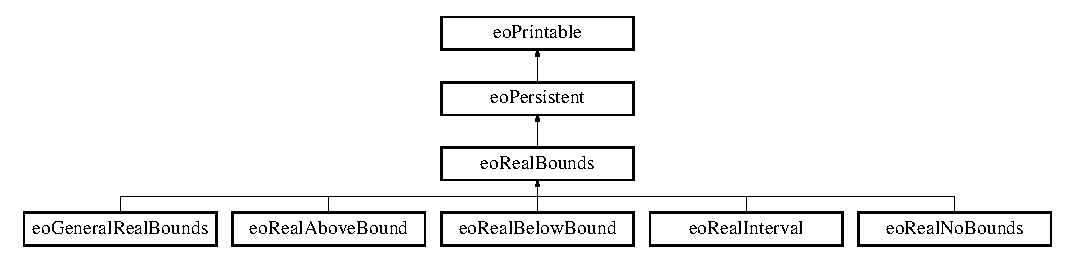
\includegraphics[height=3.06849cm]{classeo_real_bounds}
\end{center}
\end{figure}
\subsection*{Public Member Functions}
\begin{CompactItemize}
\item 
virtual bool {\bf is\-Bounded} (void) const =0\label{classeo_real_bounds_a1}

\begin{CompactList}\small\item\em Self-Test: true if $\ast$$\ast$$\ast$both$\ast$$\ast$$\ast$ a min and a max. \item\end{CompactList}\item 
virtual bool {\bf has\-No\-Bound\-At\-All} (void) const =0\label{classeo_real_bounds_a2}

\begin{CompactList}\small\item\em Self-Test: true if no min $\ast$$\ast$$\ast$and$\ast$$\ast$$\ast$ no max hence no further need to test/truncate/fold anything. \item\end{CompactList}\item 
virtual bool {\bf is\-Min\-Bounded} (void) const =0\label{classeo_real_bounds_a3}

\begin{CompactList}\small\item\em Self-Test: bounded from below??? \item\end{CompactList}\item 
virtual bool {\bf is\-Max\-Bounded} (void) const =0\label{classeo_real_bounds_a4}

\begin{CompactList}\small\item\em Self-Test: bounded from above??? \item\end{CompactList}\item 
virtual bool {\bf is\-In\-Bounds} (double) const =0\label{classeo_real_bounds_a5}

\begin{CompactList}\small\item\em Test on a value: is it in bounds? \item\end{CompactList}\item 
virtual void {\bf folds\-In\-Bounds} (double \&) const =0\label{classeo_real_bounds_a6}

\begin{CompactList}\small\item\em Put value back into bounds - by folding back and forth. \item\end{CompactList}\item 
virtual void {\bf truncate} (double \&) const =0\label{classeo_real_bounds_a7}

\begin{CompactList}\small\item\em Put value back into bounds - by truncating to a boundary value. \item\end{CompactList}\item 
virtual double {\bf minimum} () const =0\label{classeo_real_bounds_a8}

\begin{CompactList}\small\item\em get minimum value ::exception if does not exist \item\end{CompactList}\item 
virtual double {\bf maximum} () const =0\label{classeo_real_bounds_a9}

\begin{CompactList}\small\item\em get maximum value ::exception if does not exist \item\end{CompactList}\item 
virtual double {\bf range} () const =0\label{classeo_real_bounds_a10}

\begin{CompactList}\small\item\em get range ::exception if unbounded \item\end{CompactList}\item 
virtual double {\bf uniform} ({\bf eo\-Rng} \&\_\-rng=eo::rng) const =0\label{classeo_real_bounds_a11}

\begin{CompactList}\small\item\em random generator of uniform numbers in bounds ::exception if unbounded \item\end{CompactList}\item 
virtual {\bf eo\-Real\-Bounds} $\ast$ {\bf dup} () const =0\label{classeo_real_bounds_a12}

\begin{CompactList}\small\item\em for memory managements - ugly \item\end{CompactList}\end{CompactItemize}


\subsection{Detailed Description}
Defines bound classes for real numbers. 

Scalar type: ------------ Basic class is eo\-Real\-Bounds, a pure virtual.

The following pure virtual methods are to be used in mutations:\begin{itemize}
\item void folds\-In\-Bounds(double \&) that folds any value that falls out of the bounds back into the bounds, by bouncing on the limit (if any)\item bool is\-In\-Bounds(double) that simply says whether or not the argument is in the bounds\item void truncate(double \&) that set the argument to the bound value it it exceeds it\end{itemize}


So mutation can choose\begin{itemize}
\item iterate trying until they fall in bounds,\item only try once and \char`\"{}restd::pair\char`\"{} by using the folds\-In\-Bounds method\item only try once and restd::pair using the truncate method (will create a huge bias toward the bound if the soluiton is not far from the bounds)\end{itemize}


There is also a {\bf uniform()}{\rm (p.\,\pageref{classeo_real_bounds_a11})} method that generates a uniform value (if possible, i.e. if bounded) in the interval.

Derived class are {\bf eo\-Real\-Interval}{\rm (p.\,\pageref{classeo_real_interval})} that holds a minimum and maximum value, {\bf eo\-Real\-No\-Bounds}{\rm (p.\,\pageref{classeo_real_no_bounds})} the \char`\"{}unbounded bounds\char`\"{} (-infinity, +infinity) {\bf eo\-Real\-Below\-Bound}{\rm (p.\,\pageref{classeo_real_below_bound})} the half-bounded interval [min, +infinity) {\bf eo\-Real\-Above\-Bound}{\rm (p.\,\pageref{classeo_real_above_bound})} the half-bounded interval (-infinity, max]

THis file also contains the declaration of $\ast$the$\ast$ global object that is the unbounded bound 



Definition at line 75 of file eo\-Real\-Bounds.h.

The documentation for this class was generated from the following file:\begin{CompactItemize}
\item 
eo\-Real\-Bounds.h\end{CompactItemize}
